% !TEX program = xelatex
% 《通信工程综合设计III》课程设计报告
% 编译: xelatex main.tex (两遍)
\documentclass[12pt,a4paper]{ctexart}
\usepackage[margin=2.5cm]{geometry}
\usepackage{amsmath,amssymb}
\usepackage{graphicx}
\usepackage{booktabs,array,longtable,multirow}
\usepackage{xcolor}
\usepackage{tikz}
\usetikzlibrary{arrows.meta,positioning,shapes.geometric,shapes.misc,fit,backgrounds,calc}
\setlength{\headheight}{14pt}
\usepackage{listings}
\usepackage{caption}
\usepackage{enumitem}
\usepackage{fancyhdr}
\usepackage{pdfpages}
\usepackage[colorlinks=true,linkcolor=black,urlcolor=blue,citecolor=black]{hyperref}

% 全局 TikZ / 排版
% XeLaTeX + ctex：节点文本里再套 \scriptsize 时，汉字基线会相对边框上移。
% 字号只放在节点的 font 上，行盒用 strut 锁住，标注单独占空白，不压在框上。
\tikzset{
  every picture/.style={
    line cap=round, line join=round,
    execute at begin picture={\xeCJKsetup{CJKecglue={\hskip 0.12em plus 0.04em minus 0.03em}}},
  },
  every node/.style={inner sep=3.5pt, outer sep=2.5pt},
  >=Stealth,
  box/.style={draw, rounded corners=2pt, align=center, inner xsep=6pt, inner ysep=4pt,
              font=\small, execute at begin node=\strut},
  cloud/.style={box, fill=blue!8},
  edge/.style={box, fill=green!10},
  mcu/.style={box, fill=orange!10},
  proc/.style={box, fill=orange!14},
  link/.style={box, fill=green!14},
  disp/.style={box, fill=blue!10},
  lbl/.style={font=\footnotesize, align=center, fill=white, inner sep=1.5pt, outer sep=1pt},
  startstop/.style={box, rounded corners=8pt},
  process/.style={box},
  decision/.style={draw, diamond, aspect=2.5, align=center, font=\footnotesize,
                   inner sep=1pt, minimum width=26mm, minimum height=13mm,
                   execute at begin node=\strut},
  flow/.style={->, semithick},
}
\captionsetup{font=small, labelsep=quad, skip=4pt}
\setlist{nosep, leftmargin=2em, itemsep=1pt, topsep=2pt}
\linespread{1.2}\selectfont
\setlength{\textfloatsep}{8pt plus 2pt minus 2pt}
\setlength{\floatsep}{8pt plus 2pt minus 2pt}
\setlength{\intextsep}{8pt plus 2pt minus 2pt}
\setlength{\abovecaptionskip}{4pt}
\setlength{\belowcaptionskip}{2pt}


% ----- 代码样式 -----
\lstdefinestyle{ccode}{
  language=C, basicstyle=\ttfamily\footnotesize, columns=fullflexible,
  commentstyle=\color{gray}, keywordstyle=\color{blue}\bfseries,
  stringstyle=\color{red!60!black}, numbers=left, numberstyle=\tiny\color{gray},
  frame=single, framerule=0.3pt, breaklines=true, keepspaces=true,
  showstringspaces=false, xleftmargin=1.6em,
  aboveskip=6pt, belowskip=4pt,
}
\lstdefinestyle{shell}{basicstyle=\ttfamily\small, frame=single, framerule=0.3pt,
  breaklines=true, xleftmargin=1em, backgroundcolor=\color{black!4}}

\newcommand{\shotfig}[2]{% 待贴截图占位框 \shotfig{标签}{说明}
\begin{figure}[htbp]\centering
  \fbox{\parbox[c][3.2cm][c]{0.82\linewidth}{\centering\itshape 待贴截图：#2}}
  \caption{#2}\label{#1}
\end{figure}}

\pagestyle{fancy}
\fancyhf{}
\fancyhead[CE,CO]{\small 通信工程综合设计III课程设计报告}
\fancyfoot[C]{\small\thepage}
\renewcommand{\headrulewidth}{0.4pt}

\begin{document}

% 封面整页来自指导书末页的 Word 模板，由 Word 导出，不再用 LaTeX 重排。
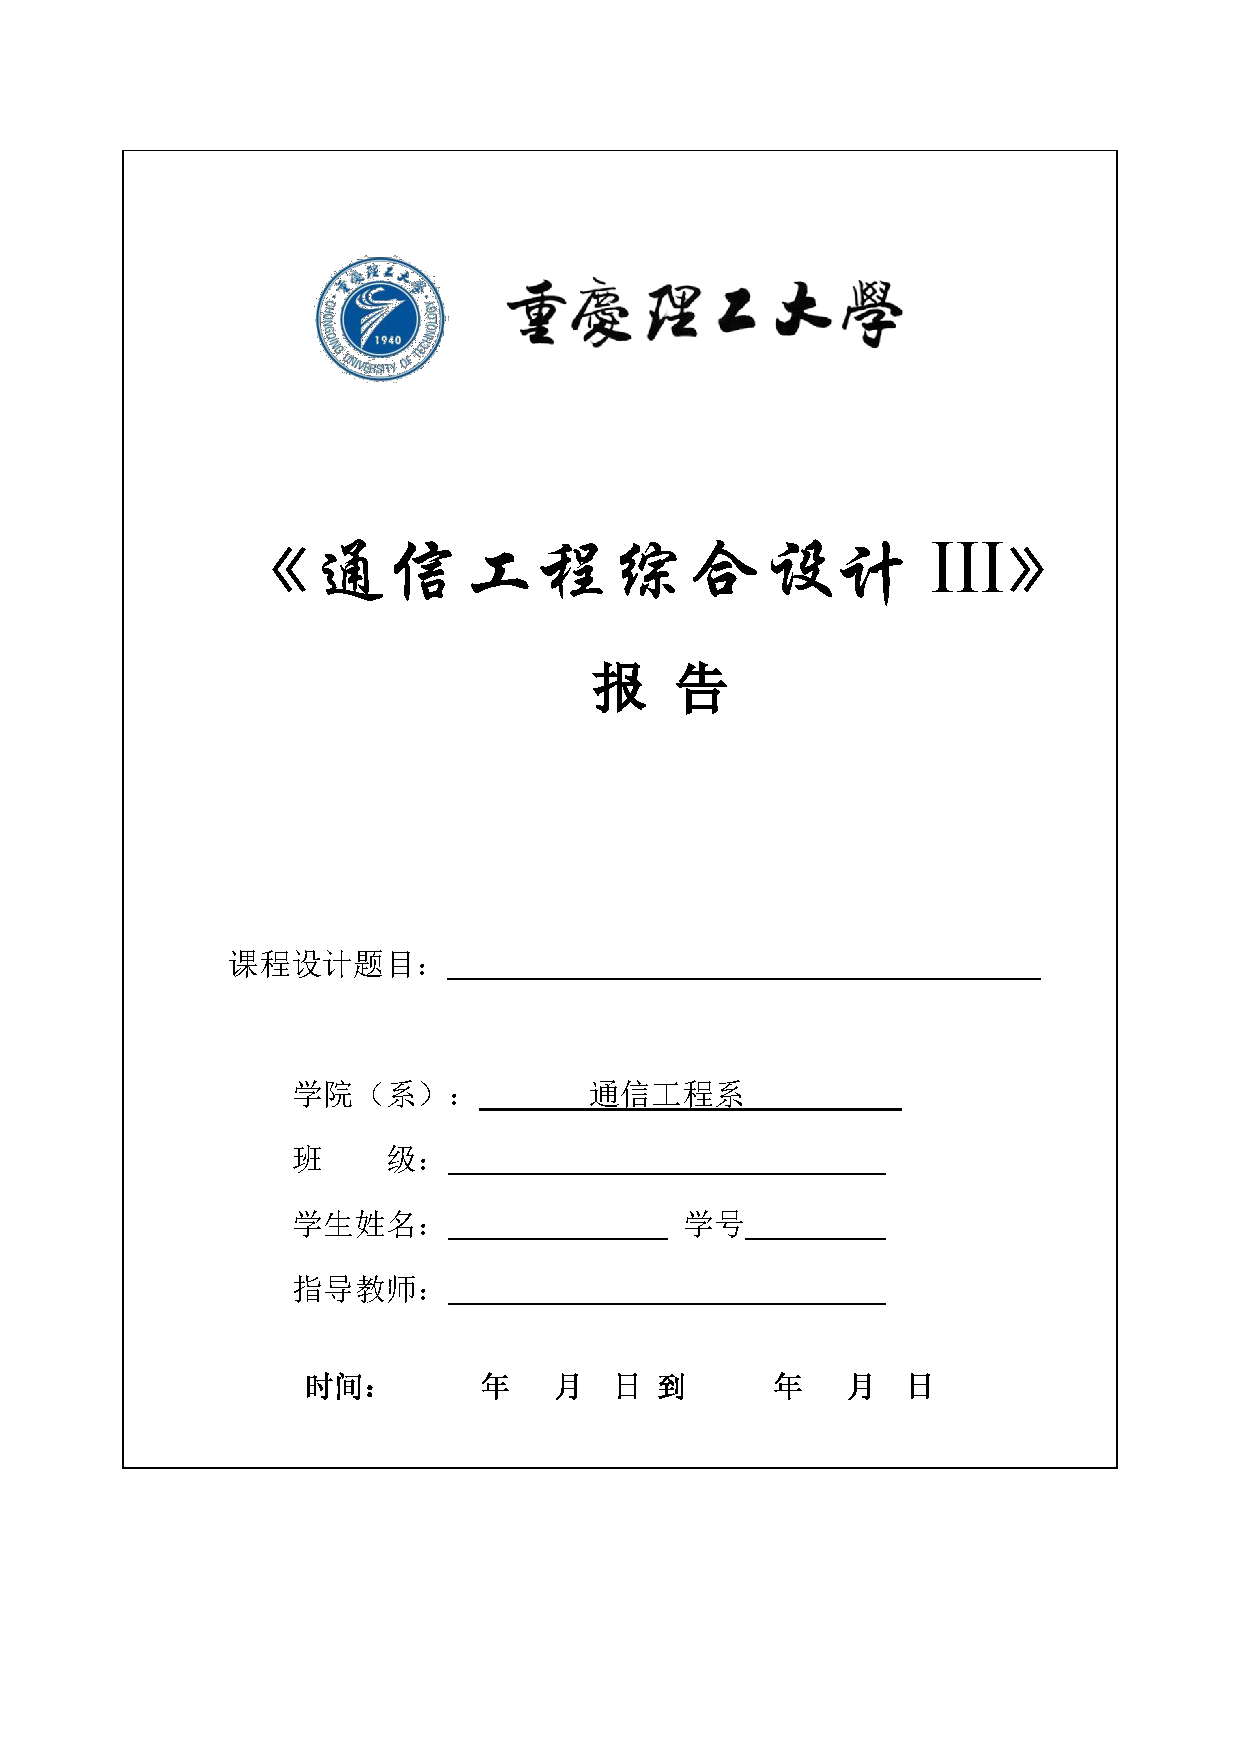
\includepdf[pages=1,pagecommand={\thispagestyle{empty}}]{fig/cover-template.pdf}
\setcounter{page}{1}

% ================= 摘要 =================
\begin{abstract}
\noindent 本设计在天马F407 开发板上实现了一个云边端协同的 AI 智能手表原型。
端侧 STM32F407ZGT6 通过 FSMC 总线驱动 3.5 寸 HX8357D 彩屏并运行 LVGL~8.3 图形界面，
在本地完成麦克风录音、MPU6050 计步与跌倒粗判、DS18B20 温度采集、RTC 走时与闹钟等功能；
边缘侧 ESP32-C3 作为通信网关，经 UART 与主控进行带 CRC 校验的自定义帧通信，
负责 Wi-Fi 连接、把 PCM 音频封装为 WAV 后通过 HTTPS 上传至云端语音大模型，
并将识别文本与天气摘要回传主控显示。语音识别采用云端大模型，本地完成指令执行，
断网时时钟、计步、测温等本地功能不受影响。F407 用 FreeRTOS 把界面刷新、
语音停等和传感器采样拆成不同优先级的任务，停等不会拖住走时和计步。
实测完成了 16\,kHz/16\,bit 录音采集、分包可靠传输、
云端语音对话与离线降级运行的完整链路。
\par\vspace{1em}
\noindent\textbf{关键词：} STM32F407；ESP32-C3；LVGL；云边端协同；AI对话；FreeRTOS
\end{abstract}
\thispagestyle{empty}
\newpage
\tableofcontents
\newpage

\section{绪论}

\subsection{选题背景与意义}
本次综合设计选题为``基于 STM32 微控制器的智能系统设计''方向，
具体实现融合了备选题目``个人语音助手''与``智能运动检测''两案要求，
以\textbf{智能手表原型}为形态组织在一块开发板上：
以语音对话作为人机交互入口，以运动计步、跌倒粗判与环境温度作为持续感知，
以彩屏表盘作为统一呈现界面。所谓``原型''，指系统当前运行在 STM32 开发板与外接模组上，
以最少的自制硬件完成完整可演示的功能闭环，验证的是架构与软件方案，而非可穿戴产品形态。

设计覆盖指导书要求的完整链条——信息采集（麦克风声音、六轴姿态、体温级温度、按键）、
信息处理与控制（STM32F407 上的计步算法、跌倒判定、语音组包与本地指令执行）、
数据传输与显示（UART 自定义帧、Wi-Fi/HTTPS 上云、LVGL 表盘）——
并在此基础上引入``云--边--端''三层协同：重负载的语音识别模型运行在云端，
嵌入式端只保留确定能在片内资源内完成、且断网也必须可用的功能。

\subsection{方案选择}
语音识别有两条技术路线：端侧小模型（关键词识别，离线可用）与云端大模型（自由问答，需联网）。
综合考虑课设周期、F407 的 168\,MHz/192\,KB RAM 算力与演示效果，
本设计采用\textbf{云边协同}路线：F407 只负责采集与可靠传输，
ESP32-C3 负责联网、TLS 与协议转换，模型推理交给云端现成的语音大模型服务。
这样端侧软件保持确定性，而交互能力上限由云端模型决定，
同时通过``断网降级''设计保证本地基础功能（走时、计步、测温）的网络无关性，
恰好形成一组可在答辩中现场演示的对照实验。

\subsection{主要工作与报告结构}
本人完成的主要工作包括：系统总体方案与云边端划分；F407 侧 FreeRTOS
任务划分与各外设驱动整合（FSMC 屏、外部 SRAM、ADC/DMA 录音、I$^2$C、单总线、RTC、WS2812 点阵）；
LVGL 六行主页与各子页，以及中文字体；F407 与 C3 之间的自定义可靠帧协议；
C3 侧语音流式上传与天气服务接入；以及覆盖主机仿真测试、烧录校验、实板联调的验证流程。

报告第 2 章为系统总体设计，第 3 章为硬件设计，第 4 章为软件与核心算法实现，
第 5 章为系统测试与效果分析，第 6 章总结与展望；
附录摘录三段开发对话，并给出核心代码节选。

\section{系统总体设计}

\subsection{需求分析}
系统需求直接来自指导书对智能系统设计题目的四项功能要求，本设计的映射关系见表~\ref{tab:req}。

\begin{table}[htbp]
\centering\small
\caption{指导书功能要求与本设计的映射}\label{tab:req}
\begin{tabular}{@{}p{4.2cm}p{5.4cm}p{4.6cm}@{}}
\toprule
指导书要求 & 本设计实现 & 承担芯片\\
\midrule
数据采集 & 麦克风录音（16\,kHz/16\,bit PCM）、MPU6050 计步与跌倒粗判、DS18B20 表温、RTC 时间、四按键 & 全部在 F407\\
本地处理/控制 & 计步算法、跌倒判定、录音组包与分包上传、闹钟/秒表/倒计时、LED 指示与蜂鸣提示 & 全部在 F407\\
GUI 界面显示 & HX8357D 上 LVGL 8.3，六行主页加时间、计步、天气、语音等子页 & F407（FSMC 总线）\\
云端交互 & 语音上传识别、天气查询，文本结果回传显示 & F407 $\to$ ESP32-C3 $\to$ 云端\\
\bottomrule
\end{tabular}
\end{table}

在四项基本要求之上，系统额外约定了三条非功能需求：
\begin{enumerate}[label=（\arabic*）]
\item \textbf{可靠性}。板间链路采用带 CRC 校验与停等重传的自定义帧协议，链路质量可统计。
\item \textbf{断网降级}。云端交互不可用时，本地走时、计步、测温、闹钟不受影响，且界面上给出明确的在线状态指示。
\item \textbf{可演示性}。全部功能可用板上四键驱动，无需额外调试器介入。
\end{enumerate}

\subsection{云边端三层架构}
系统按``云--边--端''三层划分职责，架构如图~\ref{fig:arch}所示。
划分原则是：\textbf{凡是对网络有依赖的，都放到 C3 及以上；凡是断网也必须能用的，都留在 F407。}

\begin{figure}[htbp]
\centering
\begin{tikzpicture}[node distance=10mm]
  \node[cloud, text width=12.4cm] (cloud)
    {\textbf{云端}\enspace 语音大模型（火山方舟）\enspace 天气服务（Open-Meteo）};
  \node[edge, below=of cloud, text width=12.4cm] (c3)
    {\textbf{边缘 ESP32-C3}\enspace Wi-Fi / TLS\enspace WAV 与 Base64\enspace 天气行与 JSON};
  \node[mcu, below=of c3, text width=12.4cm] (f4)
    {\textbf{端 STM32F407ZGT6}\enspace 界面、计步与跌倒、录音、测温、走时、本地指令};
  \draw[flow] (f4) -- (c3);
  \node[lbl] at ($(f4.north)!0.5!(c3.south)$) {UART4 460800，帧协议 + CRC16，双向};
  \draw[flow] (c3) -- (cloud);
  \node[lbl] at ($(c3.north)!0.5!(cloud.south)$) {HTTPS，只有 C3 联网};
\end{tikzpicture}
\caption{云边端三层架构}\label{fig:arch}
\end{figure}

各层职责边界与``不越界''约束如下：
\begin{itemize}
  \item \textbf{云}：语音大模型负责把音频变成文字回答；天气服务提供气象数据。云端不感知板级 IO，不参与计步等本地逻辑。更换云厂商时只需修改 C3 侧代码。
  \item \textbf{边（C3）}：只做网络接入与协议转换——收音频帧、补 WAV 头、调云端接口、把文本回传。不驱动屏幕、不读传感器、不做语义理解。
  \item \textbf{端（F407）}：全部采集、本地算法与显示。云端返回的文本在 F407 原样显示，不再二次解析。
\end{itemize}

\subsection{功能模块划分}
端侧软件按``采集--处理--传输--显示''四层组织，模块划分与数据流如图~\ref{fig:modules}所示。

\begin{figure}[htbp]
\centering
\begin{tikzpicture}[x=1cm, y=1cm]
  \node[box, minimum width=3.15cm] (mic) at (0,0) {麦克风\\PA5 / ADC1};
  \node[box, minimum width=3.15cm] (mpu) at (3.7,0) {MPU6050\\I$^2$C};
  \node[box, minimum width=3.15cm] (ds) at (7.4,0) {DS18B20\\PG9};
  \node[box, minimum width=3.15cm] (key) at (11.1,0) {四按键\\PA0、PE2--4};
  \node[proc, minimum width=3.15cm] (voice) at (0,-1.7) {语音状态机};
  \node[proc, minimum width=3.15cm] (pedo) at (3.7,-1.7) {计步与跌倒};
  \node[proc, minimum width=3.15cm] (slow) at (7.4,-1.7) {测温与走时};
  \node[proc, minimum width=3.15cm] (uiq) at (11.1,-1.7) {界面事件队列};
  \node[link, minimum width=14.25cm] (proto) at (5.55,-3.25)
    {帧协议：A5 5A、CRC16；音频帧停等 ACK。UART4 460800 接 ESP32-C3};
  \node[disp, minimum width=14.25cm] (lvgl) at (5.55,-4.45)
    {LVGL 8.3：六行主页与各子页。识别文本由链路任务写入，界面任务出队显示};
  \node[disp, minimum width=14.25cm] (tft) at (5.55,-5.55)
    {FSMC：HX8357D 彩屏，录音缓冲在外部 SRAM};
  \draw[flow] (mic) -- (voice);
  \draw[flow] (mpu) -- (pedo);
  \draw[flow] (ds) -- (slow);
  \draw[flow] (key) -- (uiq);
  \draw[flow] (voice.south) -- (voice.south |- proto.north);
  \draw[flow] (pedo.south) -- (pedo.south |- proto.north);
  \draw[flow] (slow.south) -- (slow.south |- proto.north);
  \draw[flow] (uiq.south) -- (uiq.south |- proto.north);
  \draw[flow] (proto) -- (lvgl);
  \draw[flow] (lvgl) -- (tft);
\end{tikzpicture}
\caption{端侧功能模块划分与数据流}\label{fig:modules}
\end{figure}


\subsection{功能设计}
\subsubsection{语音交互状态机}
语音是系统最复杂的一条业务链路，F407 侧以六状态机组织（图~\ref{fig:voicefsm}）：
按住 K\_UP 开始录音，松开或录满上限自动停止；短于 400\,ms 的按压视为误触丢弃；
上传阶段对每一音频帧执行停等式应答，超时 300\,ms 重发、最多 3 次；
END 帧获 ACK 后进入识别等待，超时 30\,s 视为失败。

\begin{figure}[htbp]
\centering
\begin{tikzpicture}[x=1cm, y=1cm]
  \node[startstop, minimum width=3.4cm] (idle) at (0,0) {空闲};
  \node[process, minimum width=3.4cm] (rec) at (0,-1.45) {录音，最长 10 s};
  \node[process, minimum width=3.4cm] (up) at (0,-2.9) {上传，停等 ACK};
  \node[process, minimum width=3.4cm] (wait) at (0,-4.35) {等待识别};
  \node[startstop, minimum width=3.4cm] (res) at (0,-5.8) {显示结果 5 s};
  \node[startstop, minimum width=3.5cm] (fail) at (6.15,-2.9) {失败后回空闲};
  \draw[flow] (idle) -- (rec);
  \draw[flow] (rec) -- (up);
  \draw[flow] (up) -- (wait);
  \draw[flow] (wait) -- (res);
  \draw[flow] (up.east) -- (fail.west);
  \draw[flow] (wait.east) -- (6.15,-4.35) -- (fail.south);
  \draw[flow] (res.west) -- (-2.55,-5.8) -- (-2.55,0) -- (idle.west);
  \node[lbl, anchor=west] at (1.95,-0.72) {按住上键};
  \node[lbl, anchor=west] at (1.95,-2.18) {满 0.4 s 才上传；更短则丢弃};
  \node[lbl, anchor=north] at (3.15,-3.08) {3 次失败};
  \node[lbl, anchor=south west] at (2.05,-4.15) {超时或 NACK};
  \node[lbl, anchor=west] at (1.95,-5.08) {收到 ASR\_TEXT};
  \node[lbl, anchor=east] at (-2.75,-2.9) {5 s 后返回};
\end{tikzpicture}
\caption{语音交互状态机}\label{fig:voicefsm}
\end{figure}

\subsubsection{语音链路时序}
一次完整的``说一句话并得到回答''过程涉及 F407、C3 与云端三方，时序如图~\ref{fig:seqvoice}所示。

\begin{figure}[htbp]
\centering
\begin{tikzpicture}[x=1cm, y=0.72cm]
  \node[proc, minimum width=2.2cm] (f4) at (0,0) {F407};
  \node[link, minimum width=2.4cm] (c3) at (6.5,0) {ESP32-C3};
  \node[cloud, minimum width=1.8cm] (cl) at (12.2,0) {云端};
  \draw (0,-0.7) -- (0,-10.3);
  \draw (6.5,-0.7) -- (6.5,-10.3);
  \draw (12.2,-0.7) -- (12.2,-10.3);
  \draw[flow] (0.15,-1.2) -- (6.35,-1.2);
  \node[lbl, above=0pt] at (3.25,-1.2) {HELLO，直到 HELLO\_ACK};
  \draw[flow] (0.15,-2.2) -- (6.35,-2.2);
  \node[lbl, above=0pt] at (3.25,-2.2) {AUDIO\_BEGIN（总字节）};
  \draw[flow] (0.15,-3.2) -- (6.35,-3.2);
  \node[lbl, above=0pt] at (3.25,-3.2) {AUDIO\_DATA，最多 506 字节};
  \draw[flow] (6.35,-4.2) -- (0.15,-4.2);
  \node[lbl, above=0pt] at (3.25,-4.2) {ACK / NACK，300 ms，最多 3 次};
  \draw[flow] (0.15,-5.2) -- (6.35,-5.2);
  \node[lbl, above=0pt] at (3.25,-5.2) {AUDIO\_END};
  \draw[flow] (6.35,-6.2) -- (0.15,-6.2);
  \node[lbl, above=0pt] at (3.25,-6.2) {ACK};
  \draw[flow] (6.65,-7.2) -- (12.05,-7.2);
  \node[lbl, above=0pt] at (9.35,-7.2) {WAV + Base64};
  \draw[flow] (12.05,-8.2) -- (6.65,-8.2);
  \node[lbl, above=0pt] at (9.35,-8.2) {JSON};
  \draw[flow] (6.35,-9.2) -- (0.15,-9.2);
  \node[lbl, above=0pt] at (3.25,-9.2) {ASR\_TEXT};
\end{tikzpicture}
\caption{语音上传与识别回传时序}\label{fig:seqvoice}
\end{figure}

\subsubsection{计步与跌倒处理流程}
计步每 20\,ms 执行一次：读三轴原始值、计算合加速度、一阶滤波跟踪重力基线、
动态分量越过阈值后回落记一步；同一会话内叠加跌倒粗判，流程如图~\ref{fig:pedoflow}。
算法细节见~4.3 节。

\begin{figure}[htbp]
\centering
\begin{tikzpicture}[node distance=5mm]
  \node[startstop, minimum width=3.2cm] (s) {每 20 ms 采样};
  \node[process, below=of s, minimum width=6.2cm] (mag) {合加速度 $mag=\sqrt{a_x^2+a_y^2+a_z^2}$};
  \node[process, below=of mag, minimum width=6.2cm] (base)
    {基线 $base \leftarrow 0.98\,base+0.02\,mag$\\动态量 $dyn=mag-base$};
  \node[decision, below=8mm of base] (cross) {越阈后回落?};
  \node[decision, below left=9mm and 8mm of cross] (gap) {间隔够?};
  \node[process, below right=9mm and 6mm of cross, minimum width=2.8cm] (hold) {保持越阈};
  \node[process, below=of gap, minimum width=2.6cm] (step) {步数加 1};
  \node[decision, below=of hold] (fall) {像跌倒?};
  \node[process, below=of fall, minimum width=3.2cm] (alarm) {蜂鸣，打开告警页};
  \draw[flow] (s)--(mag)--(base)--(cross);
  \draw[flow] (cross) -- (gap);
  \node[lbl, above left=0pt] at ($(cross.south)!0.5!(gap.north)$) {是};
  \draw[flow] (cross) -- (hold);
  \node[lbl, above right=0pt] at ($(cross.south)!0.5!(hold.north)$) {否};
  \draw[flow] (gap) -- (step);
  \node[lbl, left=1pt] at ($(gap.south)!0.5!(step.north)$) {是};
  \draw[flow] (hold) -- (fall);
  \draw[flow] (fall) -- (alarm);
  \node[lbl, right=2pt] at ($(fall.south)!0.5!(alarm.north)$) {是};
  \node[process, right=8mm of fall, minimum width=2.5cm] (again) {下一拍再判};
  \draw[flow] (fall) -- (again);
  \node[lbl, above=1pt] at ($(fall.east)!0.5!(again.west)$) {否};
\end{tikzpicture}
\caption{计步与跌倒粗判处理流程}\label{fig:pedoflow}
\end{figure}

\subsection{数据存储设计}
本系统为单机嵌入式装置，不使用服务器数据库；持久化数据全部存放在板载
EEPROM 24C02（256\,字节，I$^2$C 地址 0x50，与 MPU6050 共享总线）中，
按固定偏移组织成``数据记录表''（表~\ref{tab:ee}）。
EEPROM 读写只在慢任务中执行，避免与 20\,ms 传感器采样竞争 I$^2$C 总线。

\begin{table}[htbp]
\centering\small
\caption{24C02 数据记录表（一次读写长度 0x18 字节）}\label{tab:ee}
\begin{tabular}{@{}llp{6.9cm}@{}}
\toprule
偏移 & 长度 & 内容\\
\midrule
0x00 & 4 & 魔数 ``STEP''，作为数据有效标志\\
0x04 & 4 & 总步数（uint32，小端）\\
0x08 & 4 & 当日步数（uint32，小端）\\
0x0C & 1 & 当日对应日期（1--31），跨日清零当日步数\\
0x10 & 2 & 计步动态阈值（0.001\,g 单位，uint16），默认 150\\
0x12 & 2 & 最小步间隔（ms，uint16），默认 300\\
0x14 & 3 & 闹钟配置：使能位 + 时 + 分\\
\bottomrule
\end{tabular}
\end{table}

存储的实体关系简单（图~\ref{fig:er}）：系统配置（阈值、间隔、闹钟）与
运动记录（总步数、当日步数）两个``实体''均挂在同一 EEPROM 器件上，
通过魔数判定记录有效性；读取时任何字段越界即回写出厂默认值，
保证上电即有可用配置。

\begin{figure}[htbp]
\centering
\begin{tikzpicture}[node distance=8mm and 18mm]
  \node[cloud, text width=4.2cm] (cfg) {\textbf{系统配置}\\阈值、步间隔、闹钟\\偏移 0x10--0x16};
  \node[edge, right=of cfg, text width=4.2cm] (rec) {\textbf{运动记录}\\总步数、当日步数、日期\\偏移 0x04--0x0C};
  \node[mcu, below=14mm of $(cfg)!0.5!(rec)$, text width=5.2cm] (ee)
    {\textbf{EEPROM 24C02}\\256 字节，I$^2$C 地址 0x50\\偏移 0x00 的魔数 STEP 表示有效};
  \draw[flow] (cfg.south) -- (ee.140);
  \draw[flow] (rec.south) -- (ee.40);
\end{tikzpicture}
\caption{持久化数据都写在同一片 24C02 上，字段见上表}\label{fig:er}
\end{figure}

\subsection{界面设计}
\subsubsection{页面组织}
界面采用手机式竖排列表而不是圆表盘：主页为六行入口，子页面通过四键进入和返回，
LVGL 只重绘脏区域。页面树如下（按键：K\_UP 上移、OK/右键 进入或确认、
下键 下移、BACK/左键 返回）：

\begin{center}
\small
\begin{tabular}{@{}p{2.2cm}p{11.4cm}@{}}
\toprule
页面 & 内容与交互\\
\midrule
主页 & 六行：时间 / 计步 / 天气 / 语音 / 计算 / 游戏；焦点行 150\,ms 过渡到强调色\\
时间页 & 大字号走时；闹钟开关与对时入口；秒表与倒计时\\
计步页 & 总步数与当日步数实时显示；OK 键清零；下键进入阈值校准页\\
天气页 & C3 回传的一行中文摘要（城市/现象/温度/体感/湿度/风向）；右键循环切换城市\\
语音页 & 按住 K\_UP 说话；状态提示与云端回答文本显示\\
校准页 & 计步阈值（50--500\,mg）与步间隔四档现场标定\\
告警页 & 跌倒/闹钟/倒计时到点事件，任意键返回主页\\
秒表/倒计时页 & 1\,ms 时基计数；倒计时到点蜂鸣并弹告警\\
计算器页 & 四则运算的简易键盘页面\\
游戏菜单 & 贪吃蛇 / 乒乓 / 俄罗斯方块，进入时懒加载，BACK 退出\\
\bottomrule
\end{tabular}
\end{center}

\subsubsection{视觉与字体方案}
配色在 RGB565 下贯穿全部页面：背景 \#0B1220，正文 \#E8EEF7，
强调绿 \#3DDC97（计步数字与在线状态），告警红 \#FF5A5A，离线 \#E6B450。
脚本 \texttt{gen\_ui\_font.py} 从黑体 simhei 抽取界面用字，生成 16\,px、1\,bpp 的稀疏字体。
当前这次构建实际链入的汉字字体是 \texttt{lv\_font\_chinese\_16\_trial}，常量约 475\,KB；
Montserrat 16 与 48 另约 16\,KB 和 94\,KB，供数字、符号和大号时间。
因此 Flash 执行区约 836\,KB（上限 1\,MB），字库是大头。
片内 RAM 约 105.5\,KB / 128\,KB；10\,s 录音缓冲 320\,000\,B 放在外部 SRAM，不占这 128\,KB 里的大块。

\section{硬件设计}

\subsection{平台与器件选型}
系统硬件以天马F407 开发板为主体，外接一块 ESP32-C3 核心板作为边缘网关，
以及一只模拟麦克风模块。选型与理由见表~\ref{tab:parts}。
选型总体原则是\textbf{成本效益}：全部器件为开发板板载或十元级模组，
不自制 PCB，课设资源集中于软件与系统集成。

\begin{table}[htbp]
\centering\small
\caption{主要器件与选型理由}\label{tab:parts}
\begin{tabular}{@{}p{2.6cm}p{3.4cm}p{7.4cm}@{}}
\toprule
器件 & 型号/资源 & 选型理由\\
\midrule
主控 & STM32F407ZGT6 & Cortex-M4F@168\,MHz、1\,MB Flash、192\,KB RAM（含 64\,KB CCM），带 FPU/DSP 指令；片上外设满足 FSMC、多路 UART、ADC+DMA 需求；为本课程教学平台\\
显示屏 & 3.5 寸 HX8357D & 320$\times$480 RGB565、16 位 8080 并口，FSMC 总线直挂；断电不保存，上电即亮，无背光 GPIO\\
扩展存储 & IS62WV51216 & 512K$\times$16 位 = 1\,MB 外部 SRAM，FSMC NE3 片选；本设计将 10\,s 录音缓冲放于此处，释放内部 RAM\\
六轴传感器 & MPU6050 & 计步与跌倒检测；I$^2$C 数字接口，$\pm$2\,g 量程下灵敏度 16\,384 LSB/g；不使用 DMP，算法自研可解释\\
温度传感器 & DS18B20 & 单总线、12 位分辨率（0.0625\,$^\circ$C）；选择它是因为``表温''展示不需要高速，且单总线只占一根 PG9\\
EEPROM & 24C02 & 256\,B 掉电保存步数与配置；与 MPU6050 共享 I$^2$C，不新增器件\\
边缘网关 & ESP32-C3 核心板 & 内置 Wi-Fi 与 TLS 硬件加速，ESP-IDF 生态成熟；几元级成本；选它而非 ESP8266 的原因是 TLS/HTTP 栈维护成本和可用 RAM 明显更好\\
麦克风 & 模拟驻极体模块 & 输出 0--3.3\,V 模拟音频，直入 ADC；不需要 I$^2$S MEMS 的额外时钟线\\
\bottomrule
\end{tabular}
\end{table}

\subsection{时钟与电源}
\subsubsection{时钟树}
外部高速晶振 8\,MHz，经 PLL（分频 $M=8$、倍频 $N=336$、$P=2$）得到 168\,MHz 系统时钟。
AHB 168\,MHz、APB1 42\,MHz、APB2 84\,MHz；APB1 预分频非 1，故其上的定时器时钟翻倍为 84\,MHz。
录音采样由 TIM3 产生：$84\,\text{MHz}/5250=16\,\text{kHz}$，可整除无累积误差，
TIM3 以 TRGO 信号触发 ADC1 按采样率转换。RTC 由外部 32.768\,kHz 晶振驱动，
后备域由 VBAT 纽扣电池维持，主电断开后日历继续走时。

\subsubsection{电源}
开发板由 USB 或 5\,V 适配器供电，板上稳压输出 3.3\,V。
C3 与麦克风均从板上 3.3\,V 排针取电。需要注意 Wi-Fi 发射时 C3 电流出现数百毫安尖峰，
叠加 TFT 背光电流后，若电脑前置 USB 口供电能力不足可能导致整板复位；
演示与联调时优先使用独立 5\,V/1\,A 以上电源。

\subsection{关键接口连接}
系统接口连接汇总见图~\ref{fig:hwconn}（F407 侧引脚均为实测原理图网络名）。

\begin{figure}[htbp]
\centering
\begin{tikzpicture}[x=1cm, y=1cm]
  \node[mcu, align=left, font=\footnotesize, text width=6.15cm, minimum height=7.6cm,
        anchor=north west] (f4) at (0,0)
    {\textbf{STM32F407ZGT6}\\
     PA5 \enspace 麦克风，ADC1 通道 5\\
     PB8 / PB9 \enspace I$^2$C：MPU6050 与 24C02\\
     PG9 \enspace DS18B20，10 k$\Omega$ 上拉\\
     PA0、PE2、PE3、PE4 \enspace 四按键\\
     PF8 / PF9 / PF10 \enspace 蜂鸣、LED1、LED2\\
     PE5 \enspace 5$\times$5 WS2812，滚动 CQUT\\
     PC10 发、PC11 收 \enspace UART4 460800\\
     FSMC \enspace 屏与外部 SRAM 共用数据总线};
  \node[box, text width=5.35cm, anchor=north west] (tft) at (8.05,-0.05)
    {HX8357D 彩屏\\16 位 FSMC，NE4 = PG12\\RS = A6，基址 0x6C000000};
  \node[box, text width=5.35cm, anchor=north west] (sram) at (8.05,-2.05)
    {IS62WV51216，1 MB\\FSMC NE3 = PG10\\基址 0x68000000};
  \node[edge, text width=5.35cm, anchor=north west] (c3) at (8.05,-4.05)
    {ESP32-C3\\GPIO4 发送，GPIO5 接收\\与 F407 交叉、共地};
  \node[cloud, text width=5.35cm, anchor=north west] (net) at (8.05,-6.05)
    {Wi-Fi 与云端\\语音模型、Open-Meteo};
  \draw[flow] (f4.east |- tft.west) -- (tft.west);
  \draw[flow] (f4.east |- sram.west) -- (sram.west);
  \draw[flow] (f4.east |- c3.west) -- (c3.west);
  \draw[flow] (c3.south) -- (net.north);
\end{tikzpicture}
\caption{系统接口连接框图}\label{fig:hwconn}
\end{figure}

\subsubsection{显示与扩展存储总线}
HX8357D 的 16 位 8080 并口直接挂在 FSMC 上：片选 NE4（PG12）对应 Bank1 子区 4，
寄存器基址 0x6C000000；地址线 A6 充当 RS（命令/数据选择），16 位总线下对应
字节偏移 0x80，即命令/数据两个地址只差一位寻址。外部 SRAM 用 NE3（PG10），
基址 0x68000000，与 LCD 共享数据线和地址线、仅靠片选区分，二者可同时启用。
不设全屏帧缓冲（320$\times$480$\times$2$\approx$300\,KB 超出内部 RAM），
LVGL 采用行缓冲脏区刷新直写 GRAM（详见 4.6 节）。

\subsubsection{音频输入链路}
开发板 ADC 区跳线 J01/J4 出厂状态会把电位器、触摸、DAC 信号并联到 PA5，
接麦克风前必须拔除跳线帽。TIM3 以 16\,kHz TRGO 触发 ADC1 通道 5（PA5），
采样时间 84 周期，转换结果由 DMA 双半环缓冲搬运（详见 4.2 节）。

\subsubsection{F407 与 C3 的连接}
板载 ESP8266 座与 USART3、RS232 收发芯片处于同一对 TTL 网络，
且其 8 脚脚序按 ESP8266 定义（含 W\_RST/CH\_PD 等控制脚），与 C3 核心板不兼容，
故 C3 用杜邦线连接，不占用任何板载座：
PC10（UART4\_TX）接 C3 的 GPIO5（RX）、PC11（UART4\_RX）接 GPIO4（TX），
共地，3.3\,V 从板上排针取。波特率 460\,800\,8N1。
PC10/PC11 同时是 SDIO 的 D2/D3 复用脚，故 TF 卡必须保持不插。

\subsection{接口冲突与跳线处理}
天马F407 外设密度高，复用冲突多。设计阶段即对全部引脚做了冲突核对，
最终状态固化在表~\ref{tab:jumper}，避免运行期因复用冲突出现诡异的复位与总线竞争。

\begin{table}[htbp]
\centering\small
\caption{跳线/座子处理与复用冲突规避}\label{tab:jumper}
\begin{tabular}{@{}p{1.8cm}p{4.6cm}p{7.0cm}@{}}
\toprule
编号/位置 & 处理 & 原因（复用冲突）\\
\midrule
J01、J4 & 跳线帽全拔 & 避免电位器/触摸/DAC/PWM 音频与麦克风在 PA5 并联\\
P3、P4 & 不短接 & C3 走 UART4，不经 USART3 与 RS232；短接会把 UART4 引脚拉进 232 网络\\
ESP8266 座 & 保持空 & 脚序不兼容 C3；占用会顶住 USART3/RS232 网络\\
TF 卡槽 & 不插卡 & PC10/PC11 为 SDIO D2/D3，插卡后 SDIO 会拉住 UART4 引脚\\
摄像头 & 不插 & PG9（DS18B20）与 PC11 亦是 DCMI 引脚\\
BOOT 跳线 & BOOT0 短接 GND & 从 Flash 启动；上电进系统 Bootloader 的排查见 5.4 节\\
USB/CAN & 出厂状态 & 本系统不用 CAN\\
J2（F1 SPI） & 不短接 & 本阶段不启用板载 F103 协处理（保留为后备算力）\\
\bottomrule
\end{tabular}
\end{table}

\section{软件设计与核心算法}

\subsection{软件总体结构}
\subsubsection{F407 侧}
F407 工程基于 Keil（ARMCC5）+ HAL 库，从开发板厂商的 FSMC-TFTLCD 例程裁剪而来，
调度使用 FreeRTOS-Kernel V10.6.2，直接调用内核 API，不套 cmsis\_os。

FreeRTOS 在这里解决的是周期互相拖累的问题。界面要每 5\,ms 刷新，计步要每 20\,ms
读传感器，测温和闹钟可以 200\,ms 做一次，语音上传却会在串口上停等最多 300\,ms。
这些工作若挤在同一个主循环里，一次停等就会让走时和计步一起停住。
所以按周期拆成任务：界面任务优先级最高，而且是唯一允许调用 LVGL 的任务；
链路、传感和慢任务只向一个 16 项队列投事件，不直接改控件。
链路任务优先级次之，停等发生在它自己的时间片里。
传感、慢任务、灯阵和游戏节拍优先级相同，各自用 \texttt{vTaskDelayUntil}
对齐周期。游戏开始时再创建步进任务，退出就删除，三个游戏不必同时占栈。
游戏步进只更新逻辑，画面仍回到界面任务里画。

节拍用 SysTick，1\,ms。HAL 的毫秒时基改到 TIM6，避免和调度器抢同一个滴答。
中断优先级分组取 4 位全抢占，这是该内核版本的要求。
栈深单位是字。分配失败或栈溢出时直接停机，方便在调试器里看现场。
常驻任务六个，划分如下。

\begin{table}[htbp]
\centering\small
\caption{F407 任务划分}\label{tab:tasks}
\begin{tabular}{@{}llp{2.15cm}p{7.6cm}@{}}
\toprule
任务 & 周期 & 优先级/栈 & 职责\\
\midrule
ui & 5\,ms & 3 / 1024 & 出队刷新 LVGL，唯一允许调用 lv\_* 的任务\\
link & 5\,ms & 2 / 512 & 语音状态机、C3 帧收发与心跳、秒表和倒计时\\
sensor & 20\,ms & 1 / 512 & MPU6050 采样、计步与跌倒；每 10 步请求落盘\\
slow & 200\,ms & 1 / 512 & RTC、DS18B20、闹钟、蜂鸣 1\,s 关断、EEPROM 写入\\
gtick & 随游戏 & 1 / 128 & 按 40 / 400 / 700\,ms 唤醒对应游戏步进\\
game & 进入时创建 & 1 / 256 & 贪吃蛇、乒乓或俄罗斯方块走一步，退出即删除\\
rgb & 约 90\,ms & 1 / 256 & PE5 上 5$\times$5 WS2812 点阵循环滚动 CQUT\\
\bottomrule
\end{tabular}
\end{table}

初始化按固定顺序进行：168\,MHz 时钟、调试串口、LED 与蜂鸣的安全态、
FSMC（LCD 与 SRAM）、LVGL 与界面、传感器和 EEPROM 恢复、RTC、DS18B20、
UART4，最后创建任务并启动调度器。初始化期间 LED1 兼作阶段指示。
USART2/3 以及板载其他串口不初始化，避免复用冲突。

\subsubsection{C3 侧}
C3 使用 ESP-IDF v5.4.4。app\_main 仅做 NVS 初始化与版本横幅（固件版本、编译时间、
ELF SHA-256 前 16 位、运行分区、空闲堆），随后启动三个功能模块：
link（UART1 帧收发任务，优先级 5）、asr（音频接收/上传状态机与后台预擦除任务）、
wifi\_mgr（事件驱动连接管理）。weather 为纯函数式模块。密钥与 SSID 全部隔离在
secrets.h，不入库也不进报告。

\subsubsection{版本自检机制}
两块板分处两个工具链，板上运行的镜像与磁盘源码可能不一致，这是实板调试中的真实坑。
为此 C3 启动横幅打印 ELF SHA-256 前 16 位，F407 侧留有 printf 镜像区供调试器读取；
固件发布时以 SHA-256 哈希为唯一身份。该机制在 5.4 节的排查中直接发挥了作用。

\subsection{核心算法一：音频采集与可靠传输}
\subsubsection{\texorpdfstring{16\,kHz DMA 采集}{16 kHz DMA 采集}}
录音链路为``TIM3 定时触发 + ADC1 转换 + DMA 双半环搬运''：
TIM3 由 84\,MHz 定时器时钟分频 $5250$ 得 16\,kHz TRGO，触发 ADC1 通道 5（PA5）
以 84 周期采样时间转换；DMA 使用 2048 点环形缓冲，分为两个 1024 点半块，
半满/全满中断中把当前半块转存为 16\,bit PCM：
\[
\text{sample} = (adc - 2048) \times 16
\]
即把 12\,bit ADC 的中点搬到 0 并左移 4 位扩展为 16\,bit。
DMA 在填一个半块的同时 ISR 拷贝另一个半块，实现无丢失连续采集。
松开按键时按冻结的 NDTR 寄存器值补齐尾部不满半块。

录音缓冲不放在内部 SRAM：按 10\,s 上限需要 320\,000\,B（16\,kHz$\times$2\,B$\times$10\,s），
故 PCM 缓冲经分散加载放入外部 SRAM（0x68000000，占其 1\,MB 的 30.5\%），
内部 RAM 只保留 DMA 环形区与句柄。考虑到外部 SRAM 挂在 FSMC 上存在时序风险，
每个半字写入后立即读回核对，失败置 MIC\_ERR\_MEMORY 错误并禁止上传——
这个自检在联调中拦截过真实的 SRAM 时序问题（见 5.4 节）。

\subsubsection{分包停等传输}
上传把 PCM 划分为不超过 506\,B 的段。偏移 4\,B 加数据 506\,B 构成 510\,B 载荷；
帧头 9\,B（SOF 到 LEN）加 CRC 2\,B，音频数据帧共 521\,B。
满长 10\,s 音频为 BEGIN + 633 个 DATA + END，共 635 帧。
传输采用停等式流控：每帧发出后等待对端回显 SEQ 的 ACK，超时 300\,ms 重发原帧，
最多 3 次；对端 NACK 或 3 次超时则本次会话失败。链路层统计 crc/ore/drop/stale\_ack
四类计数并周期打印，作为通信质量指标（见 5.2 节）。

\subsection{核心算法二：计步与跌倒粗判}
计步不使用 MPU6050 的 DMP 硬件运动处理单元，算法完全自研、参数可标定可解释。
MPU6050 配置为 $\pm$2\,g 量程、50\,Hz 输出（SMPLRT\_DIV=19、DLPF$\approx$44\,Hz），
每 20\,ms 读三轴原始值，流程：
\begin{align}
mag &= \sqrt{(a_x/16384)^2+(a_y/16384)^2+(a_z/16384)^2}\\
base &\leftarrow 0.98\,base + 0.02\,mag \quad (\text{初值 }1\,g)\\
dyn &= mag - base
\end{align}
一阶滤波以慢时间常数跟踪重力与身体姿态构成的基线，动态分量 dyn 反映脚步冲击。
记步条件：$dyn$ 上穿阈值 $th$（默认 150\,mg）后回落，且回落时刻距上一步不小于
gap（默认 300\,ms）。两个参数均可通过校准页现场调整（阈值 50--500\,mg、间隔四档），
出厂值针对正常步幅与行走频率设定。

跌倒粗判叠加在同一数据流上：合加速度 $>2.0\,g$ 连续两个采样（冲击），
或 $<0.4\,g$ 持续 80\,ms（自由落体失重）后 1\,s 内出现冲击，即判定跌倒；
触发后 5\,s 静默抑制重复告警。判定成立时蜂鸣 1\,s、切换告警页。
该算法为演示性粗判，不是医疗器械级别的跌倒检测。

\subsection{核心算法三：自定义帧协议}
F407 与 C3 之间定义了一种轻量可靠帧，双方各自独立实现（C3 侧为 11 态字节流状态机），
帧结构见表~\ref{tab:frame}。

\begin{table}[htbp]
\centering\small
\caption{帧结构与字段}\label{tab:frame}
\begin{tabular}{@{}clp{7.2cm}@{}}
\toprule
字段 & 长度 & 说明\\
\midrule
SOF & 2 & 0xA5 0x5A，字节流重新同步标志\\
VER & 1 & 0x01\\
SRC/DST & 各 1 & 0xF4（F407）/ 0xC3（ESP32-C3）\\
TYPE & 1 & 帧类型，见表~\ref{tab:types}\\
SEQ & 1 & 发送方递增；应答帧回显被应答帧的 SEQ\\
LEN & 2 & 载荷字节数（小端），0--512\\
PAYLOAD & LEN & 多字节整数一律小端\\
CRC & 2 & Modbus CRC16（多项式 0xA001、初值 0xFFFF），覆盖 VER 到载荷末字节（不含 SOF）\\
\bottomrule
\end{tabular}
\end{table}

\begin{table}[htbp]
\centering\small
\caption{帧类型定义}\label{tab:types}
\begin{tabular}{@{}llp{6.2cm}@{}}
\toprule
TYPE & 名称与方向 & 载荷\\
\midrule
0x01 & HELLO（F4$\to$C3） & 空；上电后每 2\,s 一次直到获 ACK\\
0x02 & HELLO\_ACK（C3$\to$F4） & 1\,B 在线标志（后接 4\,B IPv4）\\
0x10 & AUDIO\_BEGIN（F4$\to$C3） & PCM 总字节数 u32 小端\\
0x11 & AUDIO\_DATA（F4$\to$C3） & u32 偏移 + $\le$506\,B PCM\\
0x12 & AUDIO\_END（F4$\to$C3） & 空；C3 开始上传云端\\
0x13 & ASR\_TEXT（C3$\to$F4） & UTF-8 文本，长度由 LEN 给出\\
0x20 & CMD\_WEATHER（F4$\to$C3） & 城市名 UTF-8 字节，空则用默认城市\\
0x21 & WEATHER\_RESULT（C3$\to$F4） & 一行中文摘要 UTF-8\\
0x30 & ALERT\_FALL（F4$\to$C3） & 告警事件上报\\
0x7E/0x7F & ACK / NACK & NACK 载荷 1\,B 错误码（0x01 超时 / 0x02 CRC / 0x03 未联网 / 0x04 HTTP / 0x05 空结果 / 0x06 忙）\\
\bottomrule
\end{tabular}
\end{table}

接收侧逐字节喂入状态机：搜 SOF、核对长度合法性、收满载荷后校验 CRC，
错帧静默丢弃并计数（不回 NACK，避免把错误帧放大成双向风暴）；
语音音频帧启用停等重传，其余帧为尽力而为。
设计要点是\textbf{把可靠性做在协议里}：460800\,bit/s、8N1 下，521\,B 帧的线上时间约 11\,ms。
停等窗口因此很小；重传 3 次仍失败，就应当停下来查线，而不是继续空转。

\subsection{云端接入（C3 侧）}
\subsubsection{语音上传}
C3 把 F407 送来的三段音频帧重组、暂存到专用 flash audio 分区（384\,KB，
空闲时后台预擦除扇区，接收时 4\,KB 缓冲写入）。F407 发送 AUDIO\_END 后，
C3 从分区分块读出 PCM，边生成 44\,B 标准 WAV 头、边做 Base64 流式编码并写入
HTTPS 请求体——任何时刻都不在 RAM 中保留整段 PCM/WAV/Base64/JSON，
10\,s 音频（320\,KB）在 C3 上传输的峰值内存保持在 KB 级。
请求发往火山方舟语音模型接口（模型 doubao-seed-2-0-lite，密钥不入库），
提示词约束模型``直接回应用户语音内容、回答不超过 40 个汉字''以适配手表显示。
云端返回的 JSON 经解析提取文本字段，以 ASR\_TEXT 帧回传 F407 原样显示，
F407 不再做关键词解析。失败链路区分连接失败、上传失败、HTTP 非 2xx、JSON 解析
失败四级日志，便于定位问题所在层。

\subsubsection{天气查询}
天气服务选用免密钥的 Open-Meteo。CMD\_WEATHER 帧允许携带中文城市名：
C3 先调用 Open-Meteo 地理编码接口把城市名解析为经纬度，
再请求 forecast 接口（当前温度、体感温度、湿度、风向、天气代码），
把 WMO 天气代码映射为中文（晴/多云/阴/雾/雨/雪/雷暴等），
拼装成一行固定顺序的摘要``\,城市\ 现象\ 温度$^\circ$C\ 体感\ 湿度\%\ 风向\,''回传。
默认城市写在固件配置里，F407 可循环切换重庆、北京、上海、广州、成都。

\subsubsection{Wi-Fi 管理}
wifi\_mgr 为事件驱动：掉线后每 5\,s 重连，状态变化即时以 HELLO\_ACK(在线标志)
通知 F407，由 F407 更新状态栏的``在线/离线''显示。语音会话期间暂缓天气请求，
避免两个 HTTPS 会话并发竞争内存。

\subsection{GUI 实现要点}
LVGL 8.3 使用 20 行双缓冲，每块 320$\times$20，只刷新脏矩形。
flush 经 16 位 FSMC 写入 HX8357D 的 GRAM，不建全屏帧缓冲。
界面任务每 5\,ms 调用 lv\_timer\_handler。
主页六行卡片的焦点用 150\,ms 缓动切换。按键语义按页面分发，新增页面不必改调度循环。
当前镜像里的汉字字体是 2.6 节所说的 trial 字库，不是脚本生成的那份 KB 级子集。

\subsection{系统部署}
\subsubsection{构建与烧录流程}
\begin{itemize}
  \item F407：EIDE / Keil ARMCC5，产物 Template.hex。当前镜像代码约 245\,KB，
        Flash 执行区约 836\,KB / 1\,MB，片内 RAM 约 105.5\,KB / 128\,KB，
        外扩 SRAM 中的录音缓冲 320\,000\,B。OpenOCD 0.12 + CMSIS-DAP，
        SWD 500\,kHz 烧录并核对。
  \item C3：ESP-IDF PowerShell 终端 idf.py 构建，产物 ai-watch-c3.bin；
        esptool 先以 chip-id 只读核对芯片身份再烧录，串口监视 115\,200\,bps。
  \item 版本核对：烧录后以启动横幅的 SHA-256 与本地哈希比对确认板上即磁盘版本。
\end{itemize}

\subsubsection{运行环境}
系统上电自启，无需调试器介入：F407 从 Flash 启动（BOOT0 接地），
C3 从其 flash 启动并自动连 Wi-Fi；两板通过 UART4 双绞/杜邦线连接。
演示仅需 5\,V 电源与一块已写入 Wi-Fi 凭据的 C3。

\section{系统测试与效果}

\subsection{测试环境}
\begin{table}[htbp]
\centering\small
\caption{测试环境}\label{tab:env}
\begin{tabular}{@{}p{4.2cm}p{9.6cm}@{}}
\toprule
硬件 & 天马F407（STM32F407ZGT6）+ ESP32-C3 核心板 + 模拟麦克风 + 3.5 寸 HX8357D\\
工具链 & F407：Keil ARMCC5 / EIDE、FreeRTOS 10.6.2；C3：ESP-IDF v5.4.4\\
烧录/调试 & OpenOCD 0.12.0 + CMSIS-DAP（SWD 500\,kHz）；esptool.py；串口助手 115\,200\\
主机侧仿真 & 2026-09-23，PC 上编译 F407 的 mic/voice/usart\_c3/proto，HAL 与对端 ACK 用桩代替，38 组通过\\
\bottomrule
\end{tabular}
\end{table}

主机仿真的原始输出在 \texttt{f407/build/voice\_host/result.log}。
测试程序直接编译上述四个 C 源文件，不跑 ESP32 固件。
399\,ms 的录音被丢弃，400\,ms 进入上传；
按住到 10\,s 得到 160000 个采样、320000 字节，上传进度走到 320000/320000，
ACK 之后桩返回文本 \texttt{raw reply: open light}，该次上传计时 3175\,ms。
同一份日志还记下 BEGIN 帧超时重试 3 次后失败、NACK 码 0x04，以及识别等待 8000\,ms 超时。
最后一行为 \texttt{PASS: 38 capture/protocol/state-machine cases}。
日志里的 \texttt{[c3]} 行只是桩打印的在线标志和 crc/ore/drop 计数。
这次等待时限按当时源码是 8\,s；当前固件的识别等待已改为 30\,s，两处不要混成同一次配置。

测试遵循``每步独立通过标准''的联调顺序：屏幕与界面 $\to$ 传感器 $\to$ C3 独立联网
$\to$ 双板帧链路 $\to$ 语音全链路 $\to$ 断网降级。以下逐模块给出方法与结果。

\subsection{分模块测试}
\subsubsection{界面与走时}
下面几张是按当前 LVGL 页面生成的界面示意图，不是实机拍摄。
图中的时刻、步数和天气是排版用的样子。主页是六行列表，第一行处于选中态。
\begin{figure}[htbp]
\centering
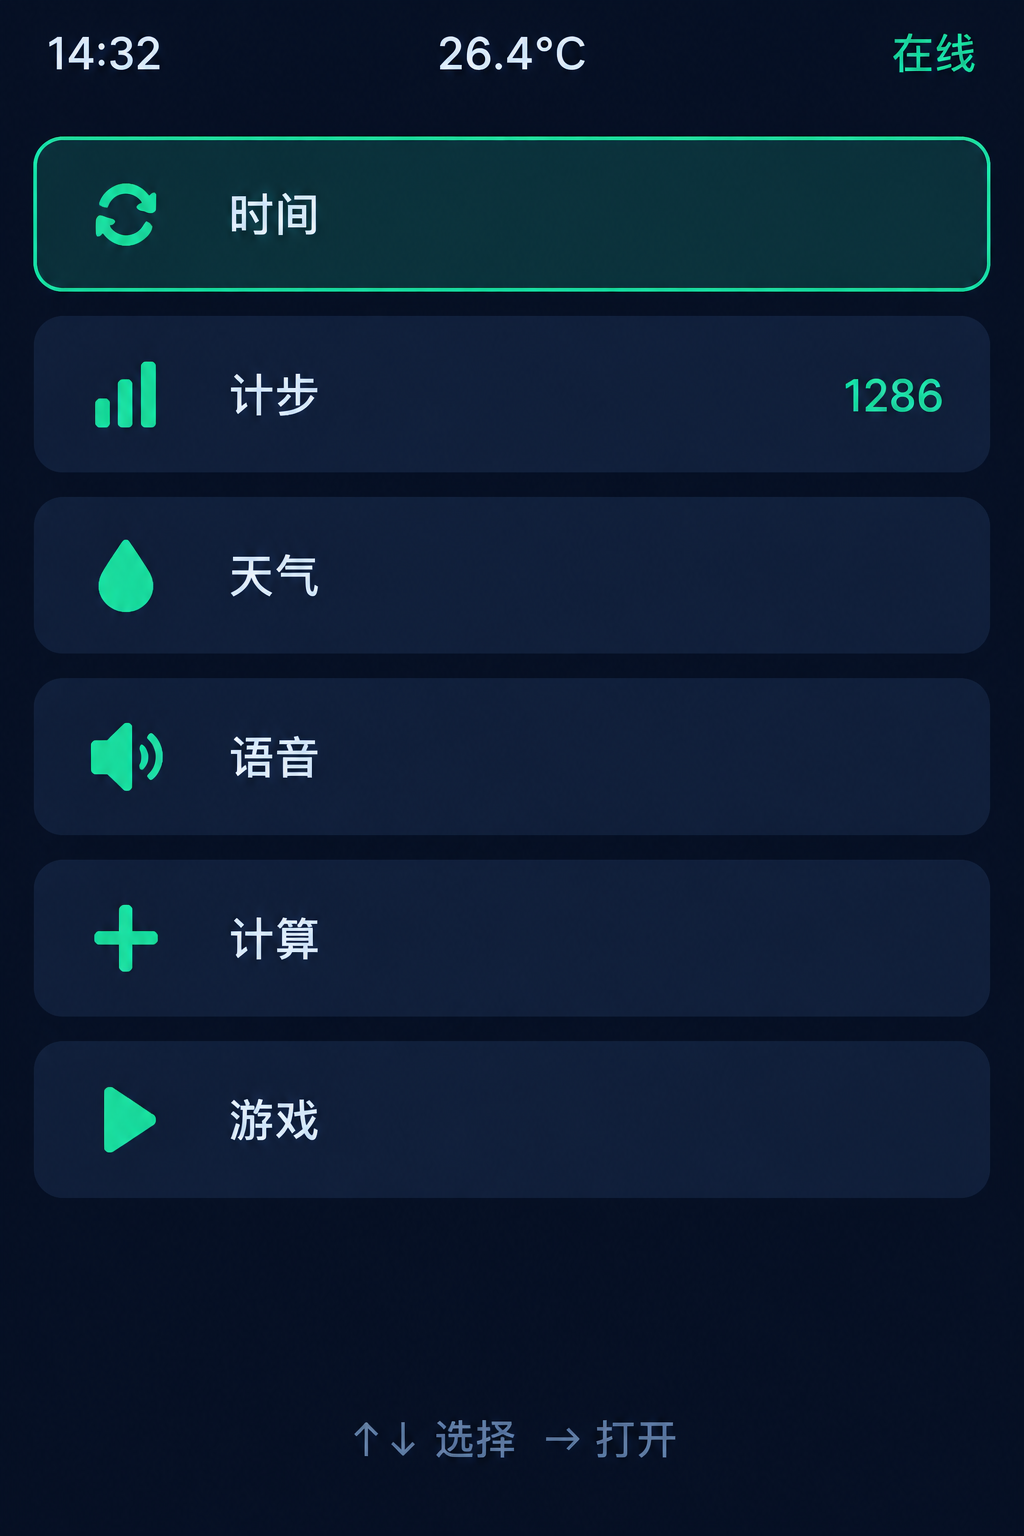
\includegraphics[width=0.36\linewidth]{picture/01.png}
\caption{主页示意图}\label{shot:home}
\end{figure}
\begin{figure}[htbp]
\centering
\includegraphics[width=0.36\linewidth]{"picture/01 (1).png"}\hfill
\includegraphics[width=0.36\linewidth]{"picture/01 (2).png"}
\caption{时间页与计步页示意图}\label{shot:time}
\end{figure}

\subsubsection{传感器与计步}
计步页已见图~\ref{shot:time}。天气页同样是示意图，摘要文字不是实测气象。
\begin{figure}[htbp]
\centering
\includegraphics[width=0.36\linewidth]{"picture/01 (3).png"}
\caption{天气页示意图}\label{shot:weather}
\end{figure}

\subsubsection{C3 串口日志}
2026-09-24 的 C3 控制台原文保存在 \texttt{dialogue\_uart.log}。\newline
固件版本是 \texttt{c3-dialogue-10s-1}。\newline
编译时间是 2026-09-24 01:16:50，ELF 校验前缀是 \texttt{adcc25215}。
启动横幅给出 UART1 为 460800\,8N1，发送脚 GPIO4，接收脚 GPIO5，
音频暂存分区 393\,216 字节、上限 320\,000 字节，启动时空闲堆 257\,264 字节。
Wi-Fi 先以 reason 4、reason 205 断开，约 5\,s 后重连，取得地址 10.95.230.254。
这条日志没有天气查询的 HTTP 记录。

\subsubsection{语音全链路}
同一份串口日志里有两段短录音，都短于 10\,s 上限。第一轮收齐后完成上云；
上传过程中又来的 BEGIN 被拒绝。第二轮只记到证书校验，文件在此结束。
\begin{table}[htbp]
\centering\small
\caption{2026-09-24 C3 串口日志中的两段语音}\label{tab:voicetest}
\begin{tabular}{@{}lcc@{}}
\toprule
项目 & 第一轮 & 第二轮\\
\midrule
PCM & 44\,502\,B & 81\,400\,B\\
串口收齐 & 1\,551\,ms & 2\,817\,ms\\
WAV & 44\,546\,B & 81\,444\,B\\
请求体 & 59\,833\,B & 109\,029\,B\\
云端 & HTTP 200 & 止于证书校验\\
HTTPS 发送 & 11\,849\,ms & 本日志没有\\
空闲堆 & 187\,740\,B & 188\,668\,B\\
\bottomrule
\end{tabular}
\end{table}
第一轮模型回复为「你好呀～请问有什么我可以帮到你的吗？」。
第二轮的 188\,668 字节是开始上传前的空闲堆。
图~\ref{shot:voice} 按该回复画了语音页，属于界面示意图。
\begin{figure}[htbp]
\centering
\includegraphics[width=0.36\linewidth]{"picture/01 (4).png"}
\caption{语音页示意图}\label{shot:voice}
\end{figure}

\subsubsection{断网降级}
关闭路由器后，状态栏右侧应由绿色「在线」改为橙色「离线」。
再按住上键时，语音页返回未联网错误（0x03）；时钟、计步和表温仍继续工作。
本报告没有单独的离线示意图。

\subsection{资源占用}
\begin{table}[htbp]
\centering\small
\caption{资源占用实测}\label{tab:resource}
\begin{tabular}{@{}llp{8.2cm}@{}}
\toprule
平台 & 资源 & 占用\\
\midrule
F407 & 代码 & 约 245\,KB\\
F407 & Flash 执行区 & 约 836\,KB / 1\,MB，其中汉字字库约 475\,KB\\
F407 & 片内 RAM & 约 105.5\,KB / 128\,KB\\
F407 & 外部 SRAM & 录音缓冲 320\,000\,B\\
C3 & 空闲堆 & 约 187\,KB\\
C3 & audio 分区 & 384\,KB，存放最长 10\,s 的 PCM\\
\bottomrule
\end{tabular}
\end{table}

\subsection{调试问题与解决过程}
调试过程记录三个有代表性的问题，全部来自真实联调，解决方式均为根因修复。

\textbf{问题一：外部 SRAM 写入偶发读回错误。}
连续录音时外扩 SRAM 出现两次 PCM 写后读校验拦截（错误码 0x20）。
排查发现 SRAM 的 FSMC 引脚配置遗漏（NE3/PG10、NBL0/NBL1/PE0/1 未初始化），
补齐引脚后仍有偶发错误，进一步把 Bank3 地址建立时间加到 3、数据建立 12 个 HCLK，
数据阶段余量约 77\,ns 后彻底消除。这一问题被自研的``写后读校验''机制当场拦截，
未产生上云的坏数据。

\textbf{问题二：复位后进入系统 Bootloader。}
一次普通复位后采样向量表，发现 MSP/PC 指向系统 ROM（0x1FFF3DA1）而非 Flash 应用，
应用未启动。逐项核对 BOOT 跳线：BOOT0 与 GND 短接确认、BOOT1 的 GND 跳线帽
脱落已补回；但补回后该次复位仍进 ROM。判断 BOOT1 与本现象无关，
真正原因是该次采样时刻 BOOT0 实际电平未被证明——USB 的 CH340 自动下载电路
亦连接 BOOT0。以调试器恢复 Flash 向量映射与 VTOR 后应用正常运行。

\textbf{问题三：板上镜像与磁盘源码不一致。}
实板日志打印的字符串既不在磁盘 C3 源码中、也不在当前构建产物中，
且 C3 收到音频帧后只回 ACK 而无云端动作——板上运行的是一份旧版固件。
据此建立了 ELF SHA-256 启动横幅自检机制，并明确``ACK 只代表帧被应答，
不代表云端请求成功''的日志语义。

\subsection{结果分析}
对照指导书要求：数据采集、本地处理与控制、GUI 显示、云端交互四项功能全部打通；
可靠性方面帧协议在两轮实测中零 CRC/零溢出/零丢帧；
断网降级行为符合设计预期。

局限与未完成项：
\begin{enumerate}[label=（\arabic*）]
\item 语音识别率未做定量验收，没有多人次、多词条的统计。
\item 麦克风存在直流偏置。录音 ADC 均值约 156，低于换算假定的中点 2048，
去均值后交流幅度偏小，云端能否听清取决于说话音量。软件里还没有去直流和增益。
\item 满 10\,s 的录音这条串口日志里没有。2026-09-24 上板的是
\texttt{c3-dialogue-10s-1}，两段都是短录音。F407 侧 10\,s 满长只做过 9 月 23 日的主机仿真。
\item 跌倒告警的 C3 上报路径（0x30 帧）已定义，尚未启用。当前只有本地蜂鸣和告警页。
\end{enumerate}

\section{总结与展望}

\subsection{完成工作}
本设计按计划交付了一个可演示的云边端协同 AI 手表原型，功能清单如下：
\begin{itemize}
  \item F407 端：LVGL 六行主页与各子页、16\,kHz/16\,bit 录音与外部 SRAM 缓冲、
        MPU6050 计步（阈值可现场改）与跌倒粗判、DS18B20 表温、RTC 与闹钟、
        秒表和倒计时、计算器、三款小游戏、EEPROM 持久化，以及 PE5 点阵滚动；
  \item C3 边缘：Wi-Fi 管理与在线上报、帧协议对端实现、PCM 流式封装 WAV 上传
        火山方舟语音模型、Open-Meteo 天气摘要、文本回传；
  \item 系统级：自定义可靠帧协议（CRC16 + 停等重传 + 链路质量统计）、
        断网降级、版本哈希自检、主机侧仿真测试集。
\end{itemize}


\subsection{收获与体会}
\begin{enumerate}[label=（\arabic*）]
\item 云边端协同的本质是\textbf{把不可靠的东西集中到一层}。网络依赖全部收敛在 C3 及以上，
F407 的软件因此保持了嵌入式应有的确定性。联调中语音链路出问题时，计步与时钟仍然稳定。
\item 自检机制的价值高于事后调试。PCM 写后读校验、CRC/ORE/DROP 计数、
SHA-256 版本横幅，各自在第一时间拦住了一类真实故障。
\item 复用冲突必须前置核对。摄像头、TF 卡、RS232、以太网等与本设计引脚冲突的资源，
全部在设计期用一张冲突表消掉，运行期没有再出现复用引发的故障。
\end{enumerate}

\subsection{展望}
\begin{enumerate}[label=（\arabic*）]
\item \textbf{音频压缩}。引入 IMA-ADPCM，把数据量压到约四分之一后再上云，
缩短 10\,s 录音的串口传输时间。
\item \textbf{端侧关键词唤醒}。在 F407 或 C3 上做离线关键词识别，
减少每次交互都要联网的等待，与云端大模型互补。
\item \textbf{跌倒上报}。启用已定义的 0x30 告警帧，把告警推送到云端或手机。
\item \textbf{产品化}。做 PCB 集成、可佩戴外形和低功耗，并考虑心率、血氧等传感。
\end{enumerate}

\appendix

\section{附录A：大模型对话摘录}
\label{app:llm}
下面三段取自开发会话。前一段是提出的改动，后一段是当时给出的改法。

\subsection{录音上限改为 10 秒}
\textbf{需求。}
定到 10 秒。如果占用太大，再上压缩算法。

\textbf{修改。}
先只改 F407：按住录音、松开停止，满 10 秒自动停，短于 400\,ms 仍丢弃。
10 秒原始 PCM 为 160000 点、320000 字节，放外部 SRAM，约占 30.5\%；
DMA 半块和外设句柄仍留在内部 SRAM。压缩先不加入，因为 C3 若整段解压再生成
WAV、Base64 和 JSON，峰值内存还在。后续若要压，优先评估 IMA ADPCM，
并同时改接收端，不能只改发送端。

\subsection{转写改为 AI 对话}
\textbf{需求。}
F407 上显示不出来。页面不要写成「识别结果」，改成「AI 对话」。
云端接的是多模态模型，提示词改为直接对语音作文字回复，不要只返回转写。

\textbf{修改。}
C3 把语音和提示词一起提交，要求用简短中文直接回应，不复述原话，
回复限制在 40 个汉字以内。协议帧类型仍用 \texttt{ASR\_TEXT}。
F407 语音页标题改为「AI对话」。当时一次真实回复用了约 11.8\,s，
而板上等待只有 8\,s，所以把磁盘源码里的等待改成 30\,s，再重新编译。

\subsection{把常用字写入片内 Flash}
\textbf{需求。}
屏幕上已经能看到回复，但有的字形没有写进单片机。
需要一份常用字较多、又能装进 ROM 的字库。

\textbf{修改。}
现有 \texttt{ui\_font.c} 只生成界面文案用到的一百多个汉字，缺字会显示成空白。
不启用 LVGL 自带的 4\,bpp 宋体，那份体积过大。
改为 16\,px、1\,bpp 的子集字库，字符先取常用汉字，再补回复里出现的标点，
英文和数字继续用 Montserrat。字模编进片内 Flash，最后以链接后的容量为准。

\section{附录B：核心代码节选}
以下为核心功能代码节选，完整工程见随报告提交的源码包。

\subsection{帧协议 CRC 与组帧（F407 proto.c）}
\lstinputlisting[style=ccode, firstline=1, lastline=60]{code/proto_excerpt.c}

\subsection{计步核心判断（F407 pedometer.c）}
\lstinputlisting[style=ccode, firstline=1, lastline=60]{code/pedometer_excerpt.c}

\subsection{DMA 录音半块转存（F407 mic.c）}
\lstinputlisting[style=ccode, firstline=1, lastline=60]{code/mic_excerpt.c}

\subsection{语音状态机推进节选（F407 voice.c）}
\lstinputlisting[style=ccode, firstline=1, lastline=60]{code/voice_excerpt.c}

\subsection{C3 帧接收状态机节选（link.c / proto.c）}
\lstinputlisting[style=ccode, firstline=1, lastline=60]{code/c3_link_excerpt.c}


\end{document}
